
\begin{figure}[!tbp]
\begin{center}
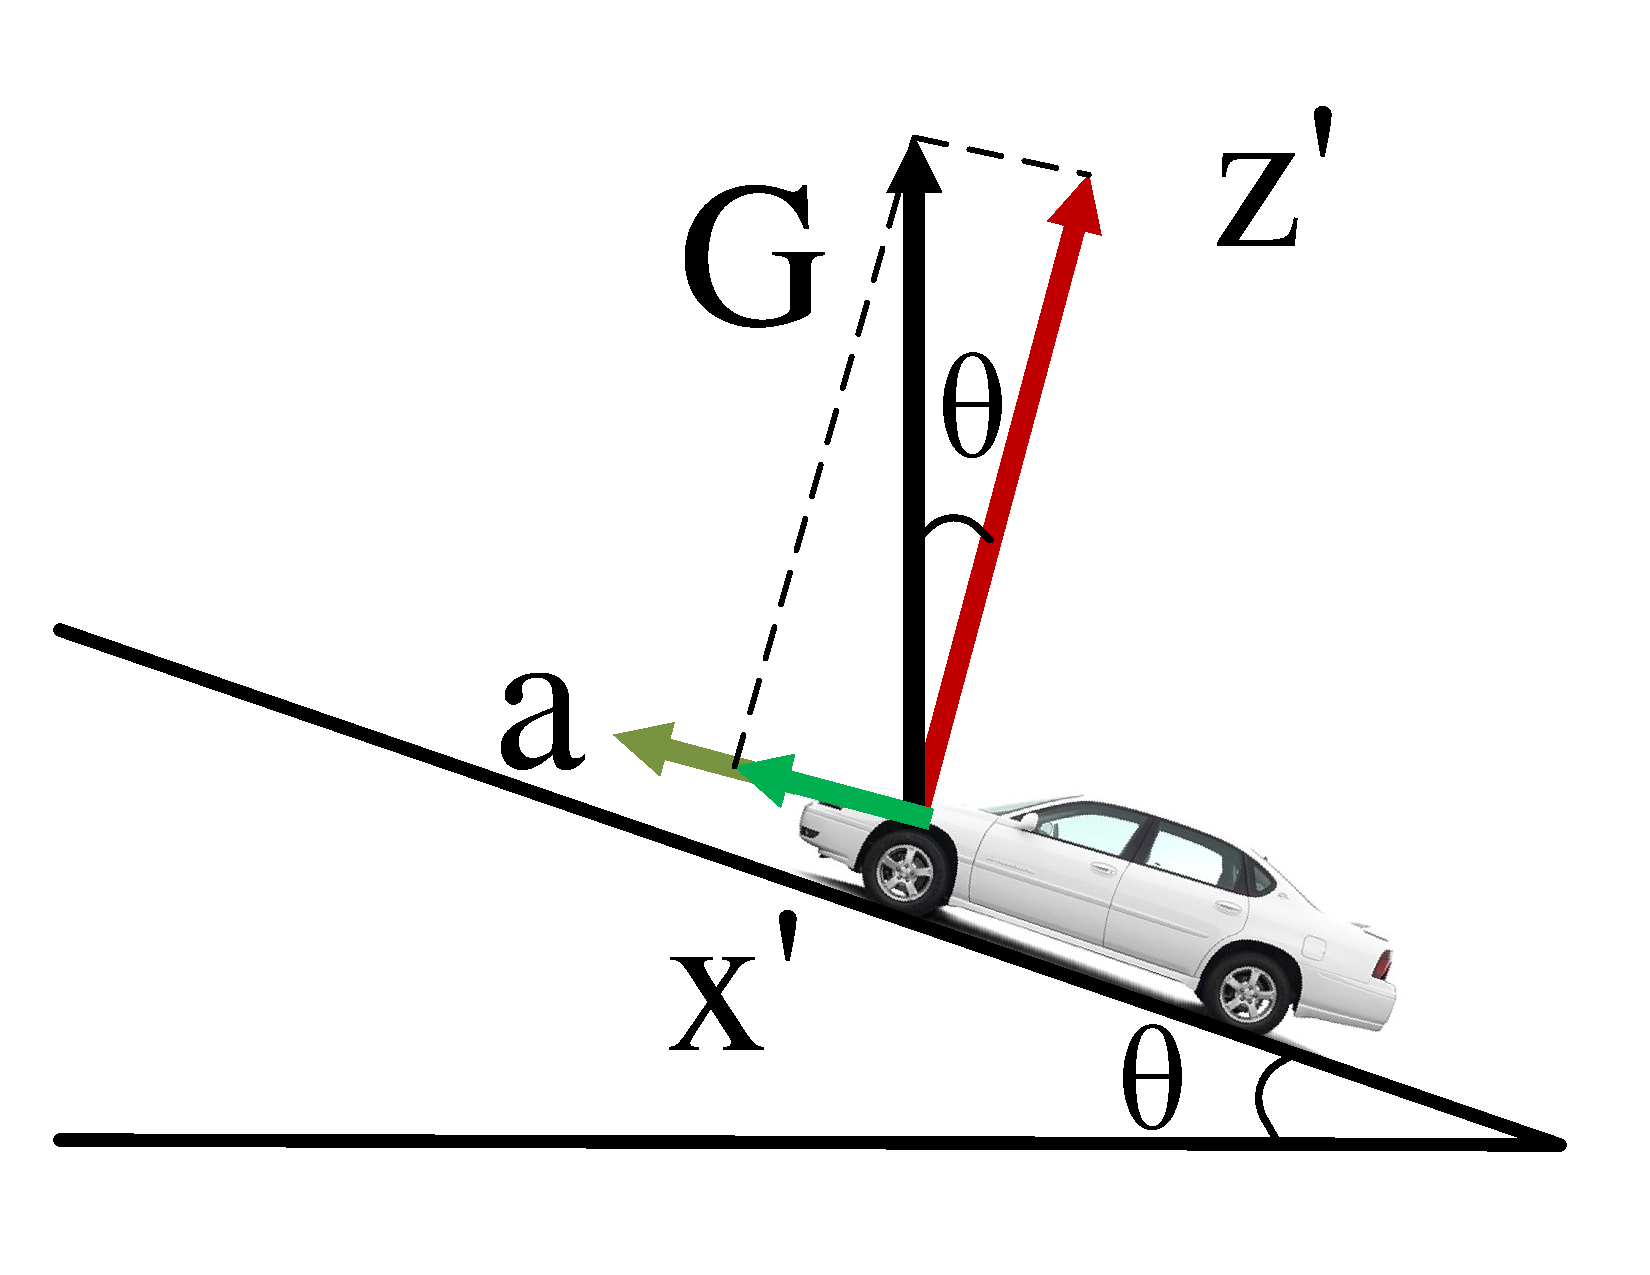
\includegraphics[width=2.0in, angle=0]{Figs/SlopeAware/slopeandcar.pdf}
\vspace{-0.0cm}
\caption{Slope gradient estimation after coordinate alignment.}
\vspace{-0.3cm}
\label{slopecar}
\end{center}
\end{figure}

After the coordinates of the smartphone and
those of the car are aligned, i.e., $[x, y, z] = [x', y', z']$, 
we can use smartphone's aligned gyroscope and accelerometer to estimate road slopes.
To estimate road segment's slope gradient,
we can track the accumulated angles along the x-axis of gyroscope. 
When the car is parked on a slope or driving over a slope,
we are able to calculate the road slope gradient according to the 
accelerometer z-axis reading and the gravity force.
An illustrative figure can be seen in Fig. \ref{slopecar}.
The slope can be calculated as $acos(z/G)$.
However, simply combining the theoretical formulas does not always work.
In followings, we discuss the various error sources that make
the slope estimation inaccurate and how to eliminate these errors
by sensor fusion. 

\subsection{Gradient Estimation by Gyroscope}


\begin{figure}[!htbp]
\begin{center}
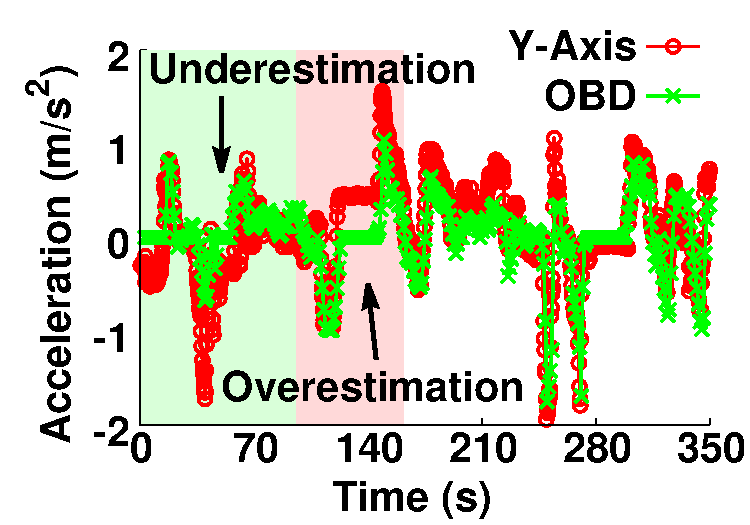
\includegraphics[width=3.5in,angle=0]{Figs/SlopeAware/accspeed.pdf}
\vspace{0.0cm}
\caption{The differences between the y-axis of the 
aligned accelerometer and the acceleration calculated from OBD data.}
\label{projectedaccelerometer}
\vspace{-0.2cm}
\end{center}
\end{figure}

\begin{figure}[!htbp]
\begin{center}
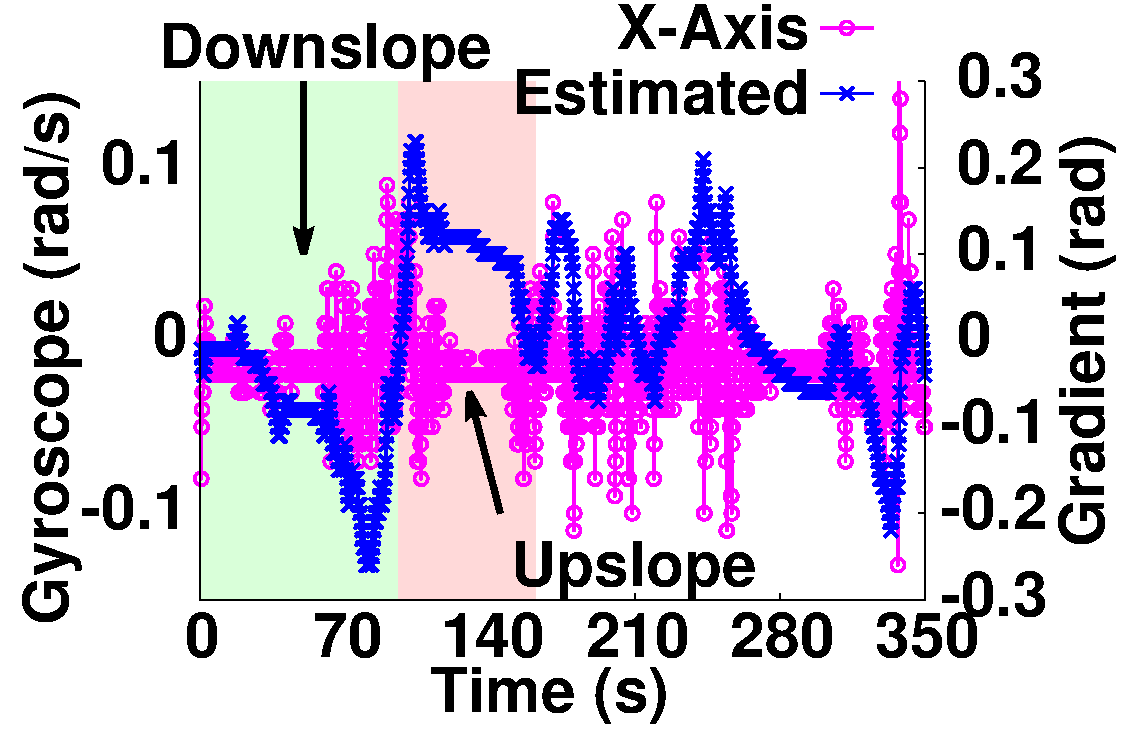
\includegraphics[width=3.5in,angle=0]{Figs/SlopeAware/gyrocompare.pdf}
\vspace{0.0cm}
\caption{Using accumulated gyroscope data to estimate slope gradients.}
\label{projectedgyroscope}
\vspace{-0.3cm}
\end{center}
\end{figure}



After coordinate alignment is done, 
we track the acceleration of a car by using the accelerometer's y-axis. 
We illustrate the acceleration values from aligned accelerometer 
in an example trip illustrated in Fig. \ref{projectedaccelerometer}. 
As the figure shows, 
the acceleration of the first $90s$ are underestimated and the next $60s$ are overestimated,
comparing with the acceleration calculated from OBD data.  
This is because the car is mainly driving downslope at 
the first $90s$ and then mainly upslope at the following $60s$. 
The deviated estimation will cause false positives/negatives on 
capturing driving behaviors such as brakes and accelerations.


We apply the same rotation matrix to the gyroscope data and 
illustrate the gyroscope x-axis data in Fig. \ref{projectedgyroscope}.
After removing the constant drifts, which we will discuss below, 
it shows clear trends that the car is driving downslope and then
upslope.
Given the similar trends illustrated in two plots, 
we can estimate the slope gradient and deduct the gravitational force
components. 
However, it requires more efforts to estimate the accurate
gradients due to various estimation errors.


\textbf{Gyroscope Estimation Errors}. 
There are mainly four reasons that cause slope estimation error by using gyroscope.  
First, the hardware precision is limited on commodity smartphones \cite{zhou2014use}.  
Second, the gyroscope drifts over time, i.e., the three-dimensional readings
are not zero even there is no rotational movement.
Third, one-dimensional readings of a phone may be affected by 
other dimensional movements of the car due
to misalignment (given that no alignment would be perfect, 
we can only increase accuracy and estimate the impacts caused by misalignment), 
e.g., the aligned x-axis may be affected by car's
z-axis movement when the car is making turns. 
Fourth, car's vibration may also cause the drift of the gyroscope.  
We use moving average function to estimate the constant drifts of a
gyroscope due to the hardware itself and the vibration of the car. 
These errors are estimated when accelerometer detects
that the car is not moving. 
The errors introduced by misalignment are very challenge to estimate, 
as the car's movements are very random, 
e.g., making turns and driving over potholes will cause different
errors on the dimension of our interest. 
To estimate these errors, we use the accelerometer to calibrate the slope estimation module.


\subsection{Calibration by Accelerometer}

\begin{figure}[!tbph]
\begin{center}
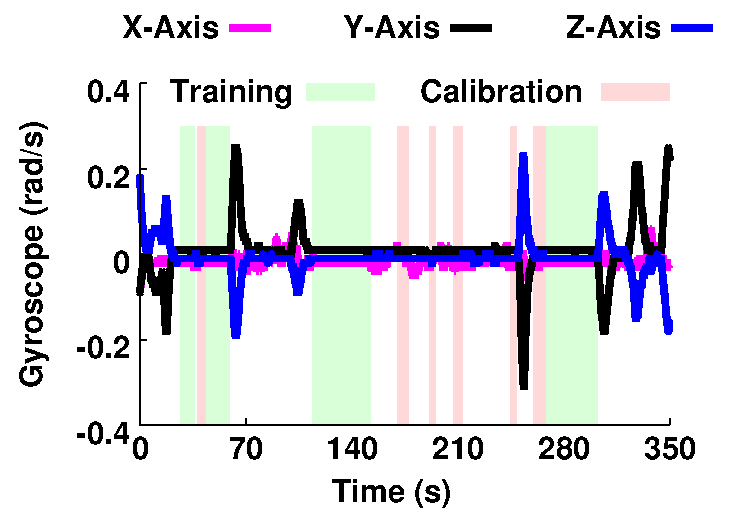
\includegraphics[width=3.5in,angle=0]{Figs/SlopeAware/training.pdf}
\vspace{0.0cm}
\caption{Selective training and calibration.}
\label{training}
\vspace{-0.3cm}
\end{center}
\end{figure}

Since the accelerometer measures acceleration and is independent 
with the gyroscope, it provides opportunities to calibrate the gyroscope.
One obvious calibration opportunity is when the 
car stopped on a slope, where we can determine
the slope gradient by $acos(z'/G)$ as illustrated in Fig. \ref{slopecar}.
However, there are two error sources for using accelerometer, 
i.e., device variance and large deviation due to misalignment.  
We normalize the gravitational forces in three dimensions
to eliminate device differences.
To eliminate the deviations caused by misalignment, 
we use the correlation of the two dimensions. 
After we eliminate the errors caused by various sources,
we combine the slope gradient tracked by gyroscope and 
accelerometer to get the linear acceleration of the vehicle. 
The result for the example trip is illustrated in Fig. \ref{linear}.

\begin{figure}[!htbp]
\begin{center}
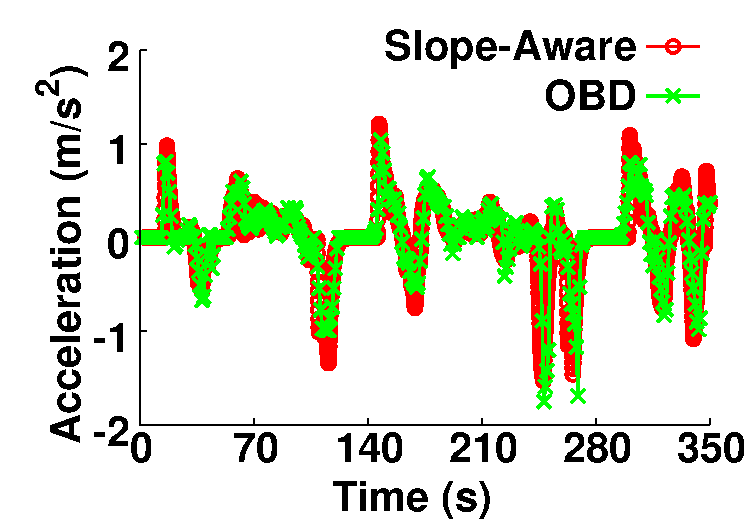
\includegraphics[width=3.5in,angle=0]{Figs/SlopeAware/acccompare.pdf}
\vspace{0.0cm}
\caption{The estimated linear accelerations by using accelerometer calibration fit better with OBD accelerations.}
\label{linear}
\vspace{-0.3cm}
\end{center}
\end{figure}


